\documentclass[12pt]{article}
\usepackage[sc]{mathpazo}
\usepackage[T1]{fontenc} 
\linespread{1.05} 
\usepackage{microtype} 
\usepackage[export]{adjustbox}
\usepackage[english]{babel} 
\usepackage[hmarginratio=1:1,top=15mm,left=15mm,columnsep=15pt]{geometry} 
\usepackage[small,labelfont=bf,up,textfont=it,up]{caption}
\usepackage{float}
\usepackage{booktabs} 
\usepackage{lettrine}
\usepackage{graphicx}
\usepackage{multicol}
\usepackage{enumitem}
\setlength{\parindent}{3ex}
\setlength{\parskip}{0ex}
\setlist[itemize]{noitemsep} 
\usepackage{abstract} 
\renewcommand{\abstractnamefont}{\normalfont\bfseries}
\renewcommand{\abstracttextfont}{\normalfont\small\itshape} 
\usepackage{titlesec} 
\renewcommand\thesection{\Roman{section}} 
\renewcommand\thesubsection{\roman{subsection}} 
\titleformat{\section}[block]{\large\scshape\centering}{\thesection.}{1em}{} 
\titleformat{\subsection}[block]{\large}{\thesubsection.}{1em}{} 
\titlespacing*{\section}
{0pt}{\baselineskip}{\baselineskip}
\setlength{\intextsep}{1ex}
\usepackage{titling} 
\usepackage{hyperref} 
\setlength{\droptitle}{-4\baselineskip}
\pretitle{\begin{center}\Huge\bfseries} 
\posttitle{\end{center}} 
\title{Problems that arise when peforming a small-scale soil microbiome analysis and how to prevent them} 
\author{
\normalsize University College London \\
}
\date{\today}
\renewcommand{\maketitlehookd}{
\begin{abstract}
\noindent 
\end{abstract}
}
\begin{document}

\maketitle
\begin{multicols}{2}
	
	
\section{Introduction}
\lettrine[nindent=0em,lines=3]{M}icrobiome analysis is an area of research that relies heavily on large samples and big amounts of data. Since the correlations between the data itself and the metadata is rarely too strong, it is important to have a wide range of samples from different biomes in order to reliably report such correlations.
\par
For that reason, one of the main areas of development in the field of microbiome analysis is the creation of a big databases with variety of samples from a range of biomes. The biggest development in this area is  EMP - Earth Microbiome Project\cite{Gilbert2014}. It was created in 2010 and focuses on creation of a global catalogue of Earth's microbial diversity, which can be used not only to perform studies on large datasets in order to find correlations within them, but also as a point of reference for criminologists and specialists in other area looking for insight into the microbial ecology of different areas.
\par
However, as with other open-source or semi open-source projects, there is always a question of how reliable and useful a single dataset can be in such a massive database? In order to test this theory, I used the genetic data of micrbes from samples of soil collected by our research group in order to test how sensible can be the data acquired from a small-scale soil analysis.
\par
The goals of the analysis were to check whether the samples we collected follow the general trends found within the EMP and to assess the small-scale result-based research in application to microbiome analysis.
%
% METHODS
%
\section{Methods}
The analysis was performed on 30 samples of soil, collected in Central London in October 2017. Metadata, such as moisture, temperature, footfall was collected on the spot, while other aspects, such as pH and concentrations of various ions was measured in the laboratory using the \textit{HI3895 Soil testing kit}. Then 4 different kits were used in a workflow designed to extract the 16S V4 DNA region from the prokaryotes in the soil, following the instructions provided by manufacturer of each kit.
\par
First, DNA was extracted using the \textit{DNeasy PowerSoil Kit} and PCR primers were designed that contained Golay barcodes, allowing multiple samples to be sequenced simultaneously. \textit{BioMic PCR kit} was used with the primers to perform the PCR. The solution acquired as the result of PCR was purified using \textit{QIAquick PCR Purification Kit} and then the concentration of dsDNA was measured using \textit{SpectraMax Quant AccuClear Nano dsDNA Assay Kit}. Using the information on DNA concentration all of the samples were subsequently diluted to equal concentrations and sequencing was performed on \textit{Illumina's MiSeq} sequencer. This workflow returned the DNA sequences that were used for downstream \textit{in silico} analysis.
\par
Analysis of sequences was performed using the QIIME\footnote{Version 1.9.1} package\cite{Caporaso2010,Kuczynski2012}, which allows users to perform high-throughput sequence analysis. Parts of analysis that required sever computational power were performed on the Cirrus High-Performance Computing system. The basic pipeline consists of:
\begin{enumerate}
	\item Data validation - checks the input data for errors
	\item Sequence demultiplexing - recognises the Golay barcodes and splits data back into 30 samples.
	\item OTU picking - for sequence analysis, it is preferable to work not with sequences directly, but with OTUs - Operational Taxonomic Units, which in our case stand for a single species.
\end{enumerate}
\par 
OTU picking requires a referencing database, for which I used SILVA\cite{Quast2012}\footnote{Release 132, April 10, 2018}, which is more up-to-date than Greengenes\cite{McDonald2012}. This pipeline sets the foundation for any further analysis and is generally the most expensive part of the analysis, in terms of computational power. For this reason it was performed on the Cirrus HPC, and most of the analysis described below was performed on a local machine. 
\par
In order to analyse our samples, I used the QIIME scripts, such as core\_diversity\_analyses.py, which allows users to take a look at basic properties of the microbial communities, such as alpha and beta diversities. However, it should be noted that while providing good results in terms of data, these workflows lack in the area of visualising data, which lead me to creation of my own visualisation scripts\cite{Anonymous2018}. They were used to validate the results of our analysis by using the data from the EMP, and points out the errors in the collected data.
\par
A method that can be useful to determine whether the samples we collected are representative of the source, is pipeline presented in the sourcetracker package\cite{Knights2011}, which allows users to track proportion of each \textit{source} in each \textit{sink}, \textit{source} and \textit{sink} being different samples of soil from Release 1 of the EMP and our samples respectively. Sourcetracker package is available with QIIME, however Sourcetracker2 has been developed recently, which was used due to being more accurate. 
\par
After filtering the data, running Sourcetracker2 and visualising the results, \textit{heatmap} of how much of each source is present in each of our samples was produced. Since hen performing such an analysis it is important to set the correct values for different parameters, such as rarefaction depth and lower threshold for number of samples an OTU can be found in, this was performed a number of times with different parameters.
\par
In an attempt to find a correlation between metadata and the diversity of our samples, scripts included in the QIIME package were used and metadata was transformed into numeric form, with results from \textit{HI3895 Soil testing kit} treated as values on exponential scale. Analysis was performed using ANOSIM\cite{CLARKE1993}, PERMANOVA\cite{Tang2016} and a collection of other statistical methods, where the distance matrix was analysed with respect to pH, potassium, nitrogen and phosphorus content.
\par
To assess the taxonomic composition of our samples, taxonomic assignment using the SILVA\cite{Quast2012} database was performed, and the uniformity of samples was assessed using visual plots that represent the proportion of each order in each sample. 
\par
In general, the analysis after the OTU picking stage was mostly performed using various python packages, such as numpy, scipy, pandas, seaborn and matplotlib, which greatly aid in data visualisation and statistical calculations.
%
% RESULTS
%
\section{Results} 
During the OTU picking stage, over 4.5 million sequences were recovered from raw data, with 16448 of them being unique. However, it should be noted, that due to use of closed-reference OTU picking, almost 800 thousand sequences (17\%) were removed from the downstream analysis since no match was found in the databases. 
\begin{figure}[H]
	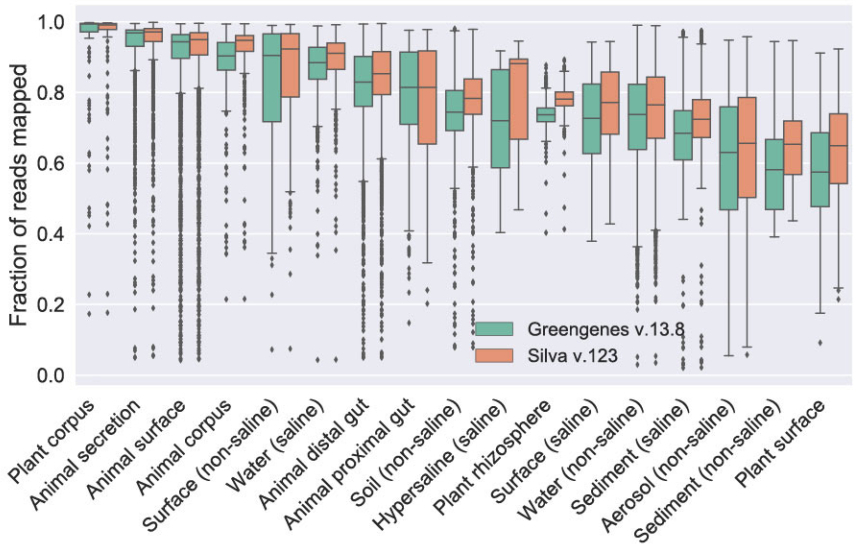
\includegraphics[width=1\linewidth]{./figs/EMP_SILVA.jpg}
	\caption{Comparison of Greengenes with SILVA databases, with number of reads in EMP samples, grouped by environment. Boxplots show median, IQR, and 1.5 × IQR (with outliers). Adapted from \cite{Thompson2017}}
	\label{fig:EMP_Silva}
\end{figure}
This result is similar to the one that was obtained on the larger-scale analogue of this research performed by Thompson et al.\cite{Thompson2017}, pictured in the Figure \ref{fig:EMP_Silva}.

Because these sequences were not found in the database, it can be assumed that they could have severely influenced diversity of the samples.
It can be noticed from Table 1, that there is no significant correlation between any of the metadata categories and diversity, since the R-value is close to zero. Other methods of statistical analysis provided similar results (not presented here).. However, similar large-scale analyses reported that there is a correlation between richness and diversity and pH\cite{Thompson2017,Fierer2006,Wu2016}.  Most likely this happened due to low number of samples and low diversity of samples (all collected from the same biome).
\begin{table}[H]
	\begin{center}
		\label{tab:table_correlation}
		\begin{tabular}{c|c|c}
			\textbf{Category} & \textbf{R-value} & \textbf{p-value}\\
			\hline
			pH & -0.109 & 0.869\\
			Potassium & 0.224 & 0.023\\
			Nitrogen & 0.120 & 0.120 \\
			Phosphorus & 0.201 & 0.058\\
		\end{tabular}
		\caption{Correlation between metadata and beta-diversity, calculated using ANOSIM\cite{CLARKE1993} methodic.}
	\end{center}
\end{table}
\par
In order to assess the composition of each sample, results from the sourcetracker analysis are presented in Figure \ref{fig:sourcetracker_heatmap}. It can be seen that most samples show highest relatedness to 3 different biomes - national park soil, field soil and agricultural soil, which is consistent with what would be expected. Sample \textit{515rcbc20} had to be excluded from the analysis due to having a very low number of OTUs observed (653), which prevents sourcetracker from producing sensible results, however the uniformity and good clustering of the rest of the samples is indirectly confirmed by this test as well. If the sample size was larger, the outliers and strange correlations, such as high proportion of wetland source in many samples could be explained, however it is impossible on this sample.
\begin{figure}[H]
	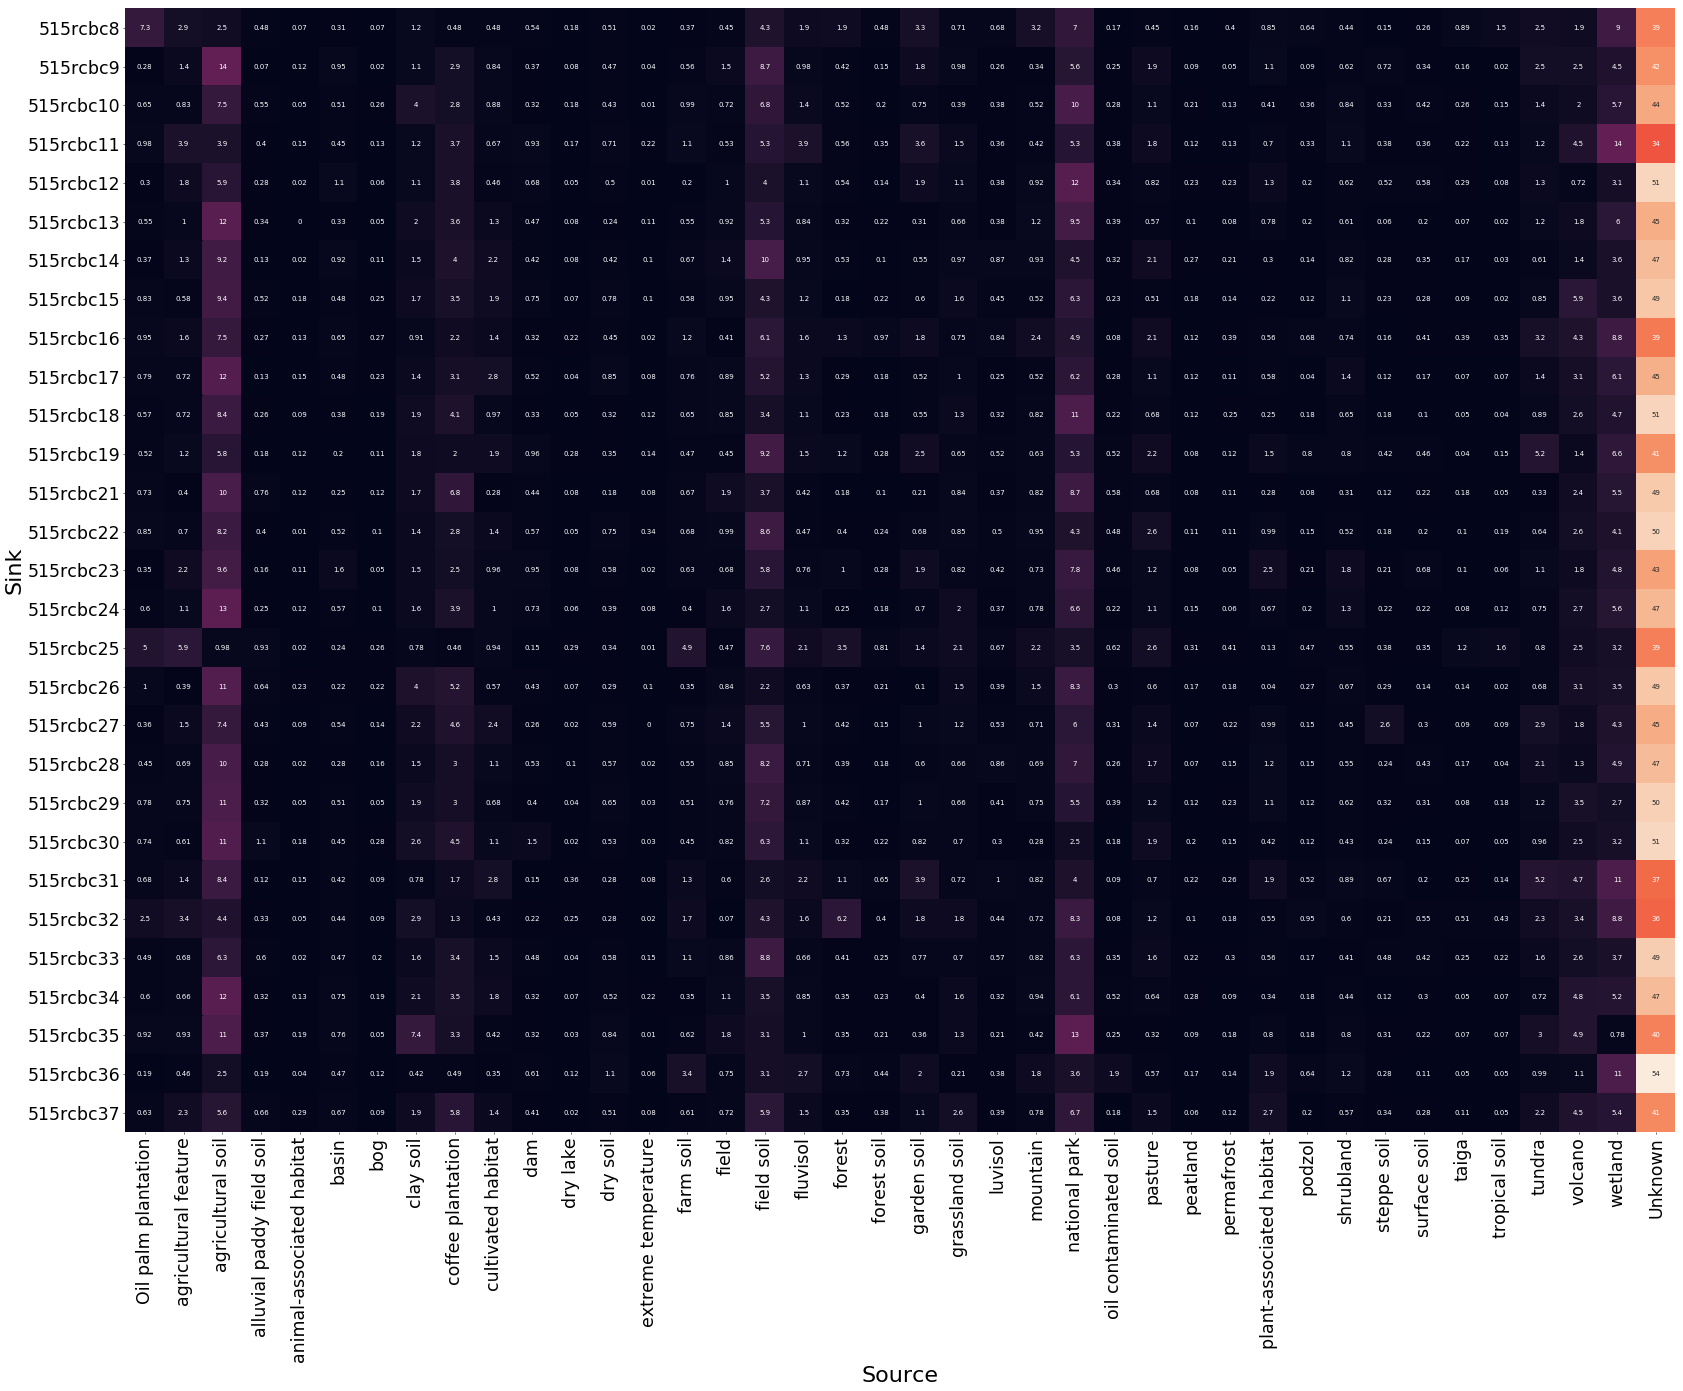
\includegraphics[width=\linewidth]{../sourcetracker/heatmap_perc.png}
	\caption{Heatmap showing the prcentage of each source in each sink. The sum of values for each sample (rows) is not equal to 100\% because the "Unknown" row is not shown here. As we can see there are 4 prominent sources in most sinks - agricultural soil, national park soil, field soil and wetland soil.}
	\label{fig:sourcetracker_heatmap}
\end{figure}
\par
Another way to assess uniformity of the samples is the alpha diversity analysis, which assesses the number of unique OTU for each sample. 
While different methods can be used, I chose the Chao1 metric, which estimates species richness based on a matrix of abundance data. 
The alpha diversity is presented below (Fig. \ref{fig:alpha_diversity}) and shows the 2 outlying samples - 515rcbc12 and 515rcbc20 having an unusually high and low alpha-diversity respectively.
\begin{figure}[H]
	\captionsetup{width=\linewidth}
	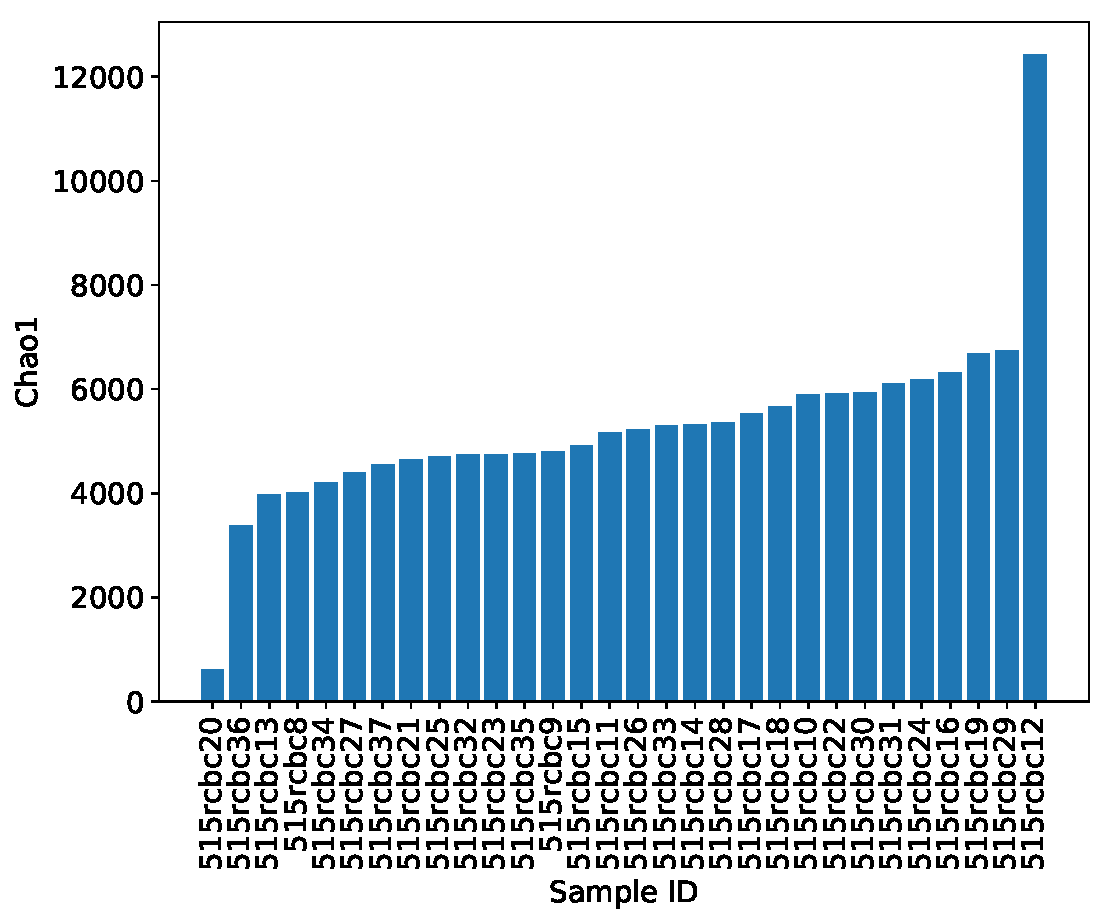
\includegraphics[width=\linewidth]{../analyses/figs/chao1_alpha.pdf}
	\caption{Alpha diversity (Chao1) for each of 30 samples.Samples 515rcbc20 and 515rcbc12 are outliers, which is could be du to the fact that they were collected outside the main location of analysis (Gordon Square in Central London), in soil near canal and compost respectively.}
	\label{fig:alpha_diversity}
\end{figure}

\par
The beta-diversity matrix showcases the difference in richness between the samples. The heatmap presented on Figure \ref{fig:beta_diversity} 

\begin{figure}[H]
	\captionsetup{width=\linewidth}
	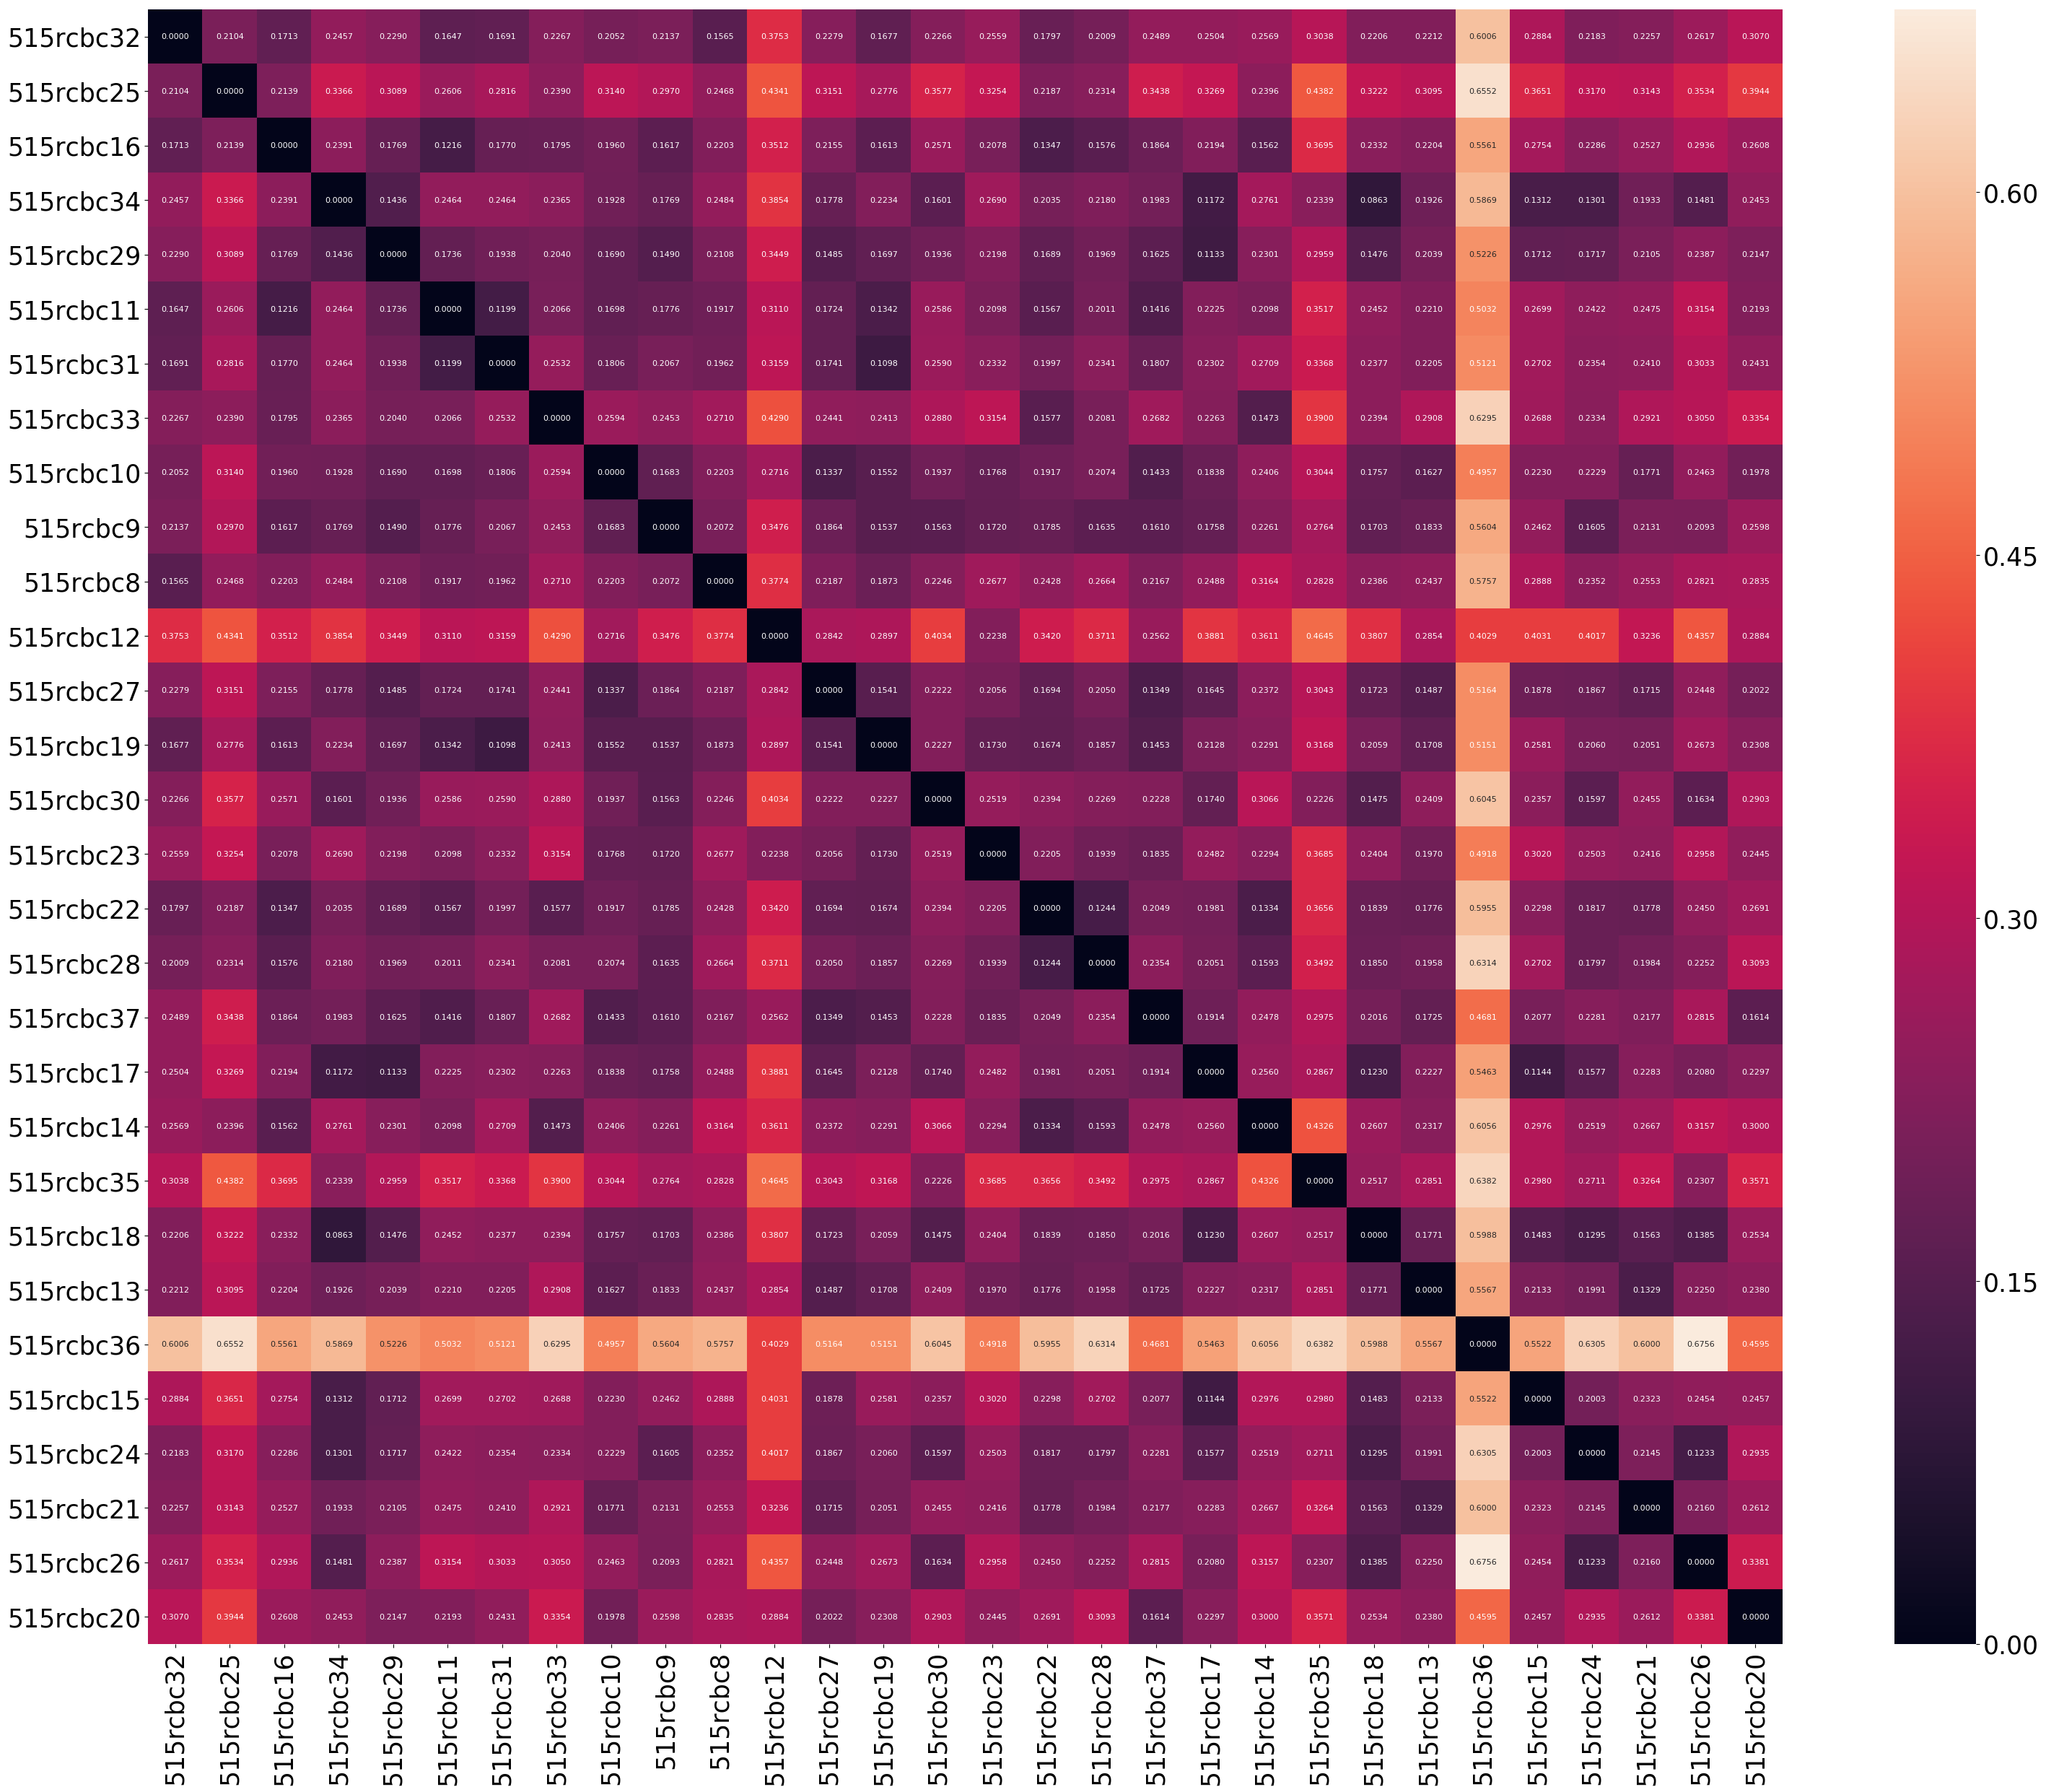
\includegraphics[width=\linewidth]{../analyses/figs/unweighted_beta.png}
	\caption{Beta diversity (unweighted unifrac). Obvious outliers can be noted again, with samples 515rcbc12 and 515rcbc36 having the largest distances from other samples.}
	\label{fig:beta_diversity}
\end{figure}




\begin{figure}[H]
	\captionsetup{width=\linewidth}
	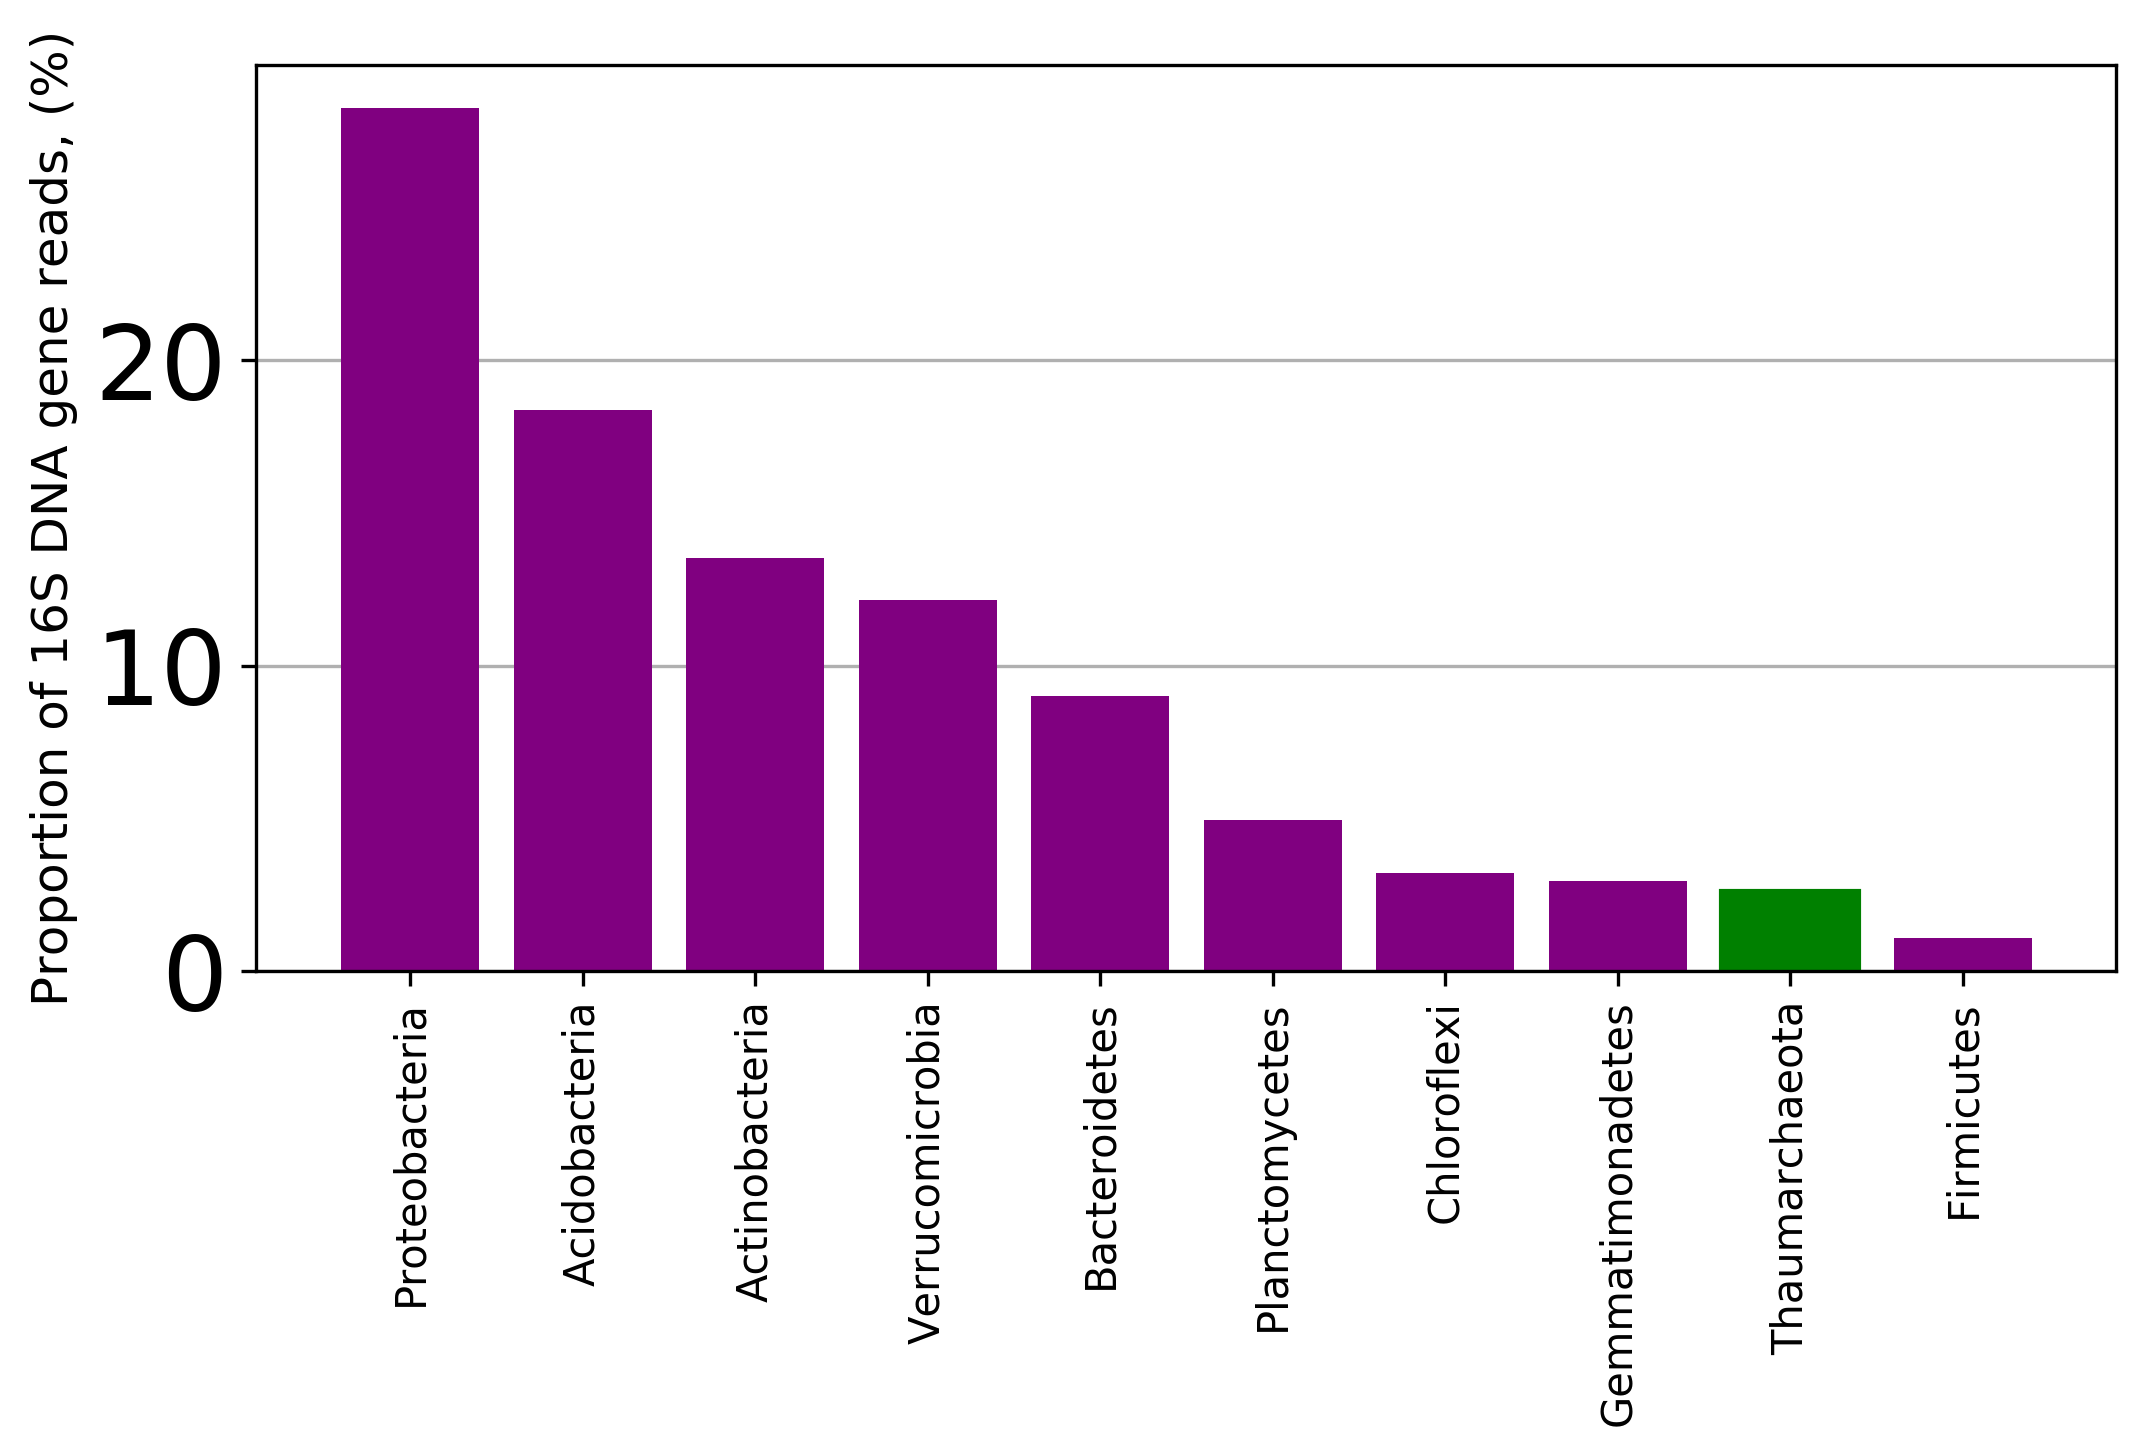
\includegraphics[width=\linewidth]{../taxonomy/top_10.png}
	\caption{Proportion of most popular phyla in samples. The green bar represents the only phylum from the Archea domain. These 10 phyla represent 96\% of species in our samples.}
	\label{fig:top_taxa}
\end{figure}
%
% DISCUSSION
%
\section{Discussion}
OTU picking strategy is outdated, and with increase of computational power and decrease in price of core-hours of High Performance Computer clusters, other techniques (for example Deblur\cite{Amir}) will provide more accurate results.
\par

Another issue that I can point out with the OTU picking method, is the limitations imposed by the databases. SILVA database currently contains 177222 sequences, which means that our study, while being rather small, already covered almost 10\% of the database. Thompson et al.\cite{Thompson2017} report that a study they performed using just under 100 samples from different biomes covered up to 50\% of the databases.

\newpage
\bibliographystyle{vancouver}
\bibliography{/home/ilya/Documents/Citations/3301.bib}
\end{multicols}
\end{document}
